\documentclass[english,twocolumn]{article}
\usepackage[T1]{fontenc}
\usepackage[latin1]{inputenc}
\usepackage{times}
\usepackage{babel}
\usepackage[letterpaper,noheadfoot,top=1.5cm,left=1.9cm,right=1.9cm,bottom=1in,columnsep=1.4cm]{geometry}
\usepackage{graphicx}

\newcommand{\fig}[4][tbp]{
  \begin{figure}[#1]
    {\centering{\includegraphics[#4]{fig/#2}}\par}
    \caption{#3}
    \label{fig:#2}
  \end{figure}
}

\begin{document}

\title{Application-Specific Communication Systems for Clusters}
\author{Ant�nio Augusto Fr�hlich\\
  \small{Laboratory for Software/Hardware Integration, Federal University of Santa Catarina}\\[-0.5ex]
  \small{88040-900 Florian�polis - SC, Brazil}\\[-0.5ex]
} 

\date{}
\maketitle
\thispagestyle{empty}
\pagestyle{empty}

\begin{abstract}

Several communication systems that claim to support high performance
computing in clusters focus on ``the best'' solution for a given
host/network architecture. However, a definitive best solution,
independently of how fine-tuned to the underlying hardware it is, cannot
exist, whereas parallel applications simply communicate differently. In
this paper, we describe a design method that enables the construction of
communication systems as an assemblage of adaptable components that can
be configured to closely match the demands of given applications. We
also describe the deployment of this method in the
\textsc{Epos} project, which delivers automatic-generated,
application-tailored runtime support systems, including a communication
system for the \textsc{Myrinet} high-speed network.

\end{abstract}

\textbf{Keywords:} runtime system design, cluster computing, user-level
communication.

\section{Introduction}

% - Cluster computing X communication

The parallel computing community has been using clusters of commodity
computers as an alternative to expensive massively parallel processors
for several years by now. The results obtained meanwhile, both positive
and negative, usually lead to the same element: inter-node
communication. This fact has encouraged enormous efforts to improve
communication performance in these clusters. From the hardware point of
view, high-speed networks and fast buses yield low-latency and
high-bandwidth, while from the software point of view, \emph{user-level
communication}~\cite{Bhoedjang:1998} enables applications to access the
network without operating system intervention and significantly reduces
the software overhead on communication. Combined, these advances left
behind the giga-bit-per-second, application-to-application communication
bandwidth barrier.

% - Criticize rigid design
%   - AM, FM, RC are target at specific communication patterns
%   - Fail to deliver comparable performance with real applications
% - Suggest application-orientation
%   - Generic X Optimum {Preikschat:1994}

Nevertheless, good communication performance is hard to obtain when
dealing with anything but the test applications supplied by the
communication package developers. Real applications, not seldom, present
disappointing performance. We believe this performance drawback to
originate in the attempt of delivering generic communication
solutions. Most high performance communication systems are looking for
``the best'' solution for a given architecture. However, a definitive
best solution, independently of how fine-tuned to the underlying
architecture it is, cannot exist, whereas parallel applications simply
communicate in different ways. Aware of this, many communication
packages claim to be ``minimal basis'', upon which application-oriented
abstractions can (have to) be implemented. Once more, there cannot be a
best minimal basis for all possible communication strategies. 

If applications communicate in different ways, we have to deliver each
one a tailored communication system that satisfies its requirements, and
nothing but its requirements. Of course we cannot implement a new
communication system for each application, what we can do is to design
the communication system in such a way that it can be tailored to any
given application. In the \textsc{Epos}
project~\cite{Froehlich:2001} we developed a novel design method
that is able to accomplish this duty. \textsc{Epos} consists of a
collection of components, a component framework, and tools to support
the automatic construction of a variety of runtime systems, including
complete operating systems. This paper focuses on \textsc{Epos}
communication system, which has been implemented for a cluster of PCs
interconnect by a \textsc{\textsc{Myrinet}} high-speed network.


\section{Application-Oriented Design}

\emph{Application-Oriented System Design} (AOSD) is a novel system design
method that, as the name suggests, has a strong compromise with
applications. Its main goal is to produce runtime support systems that
can be tailored to fulfill the requirements of particular
applications. Accomplishing this task begins with the decomposition of
the problem domain in abstractions that are natural to application
programmers. This is exactly the decomposition strategy promoted by
\emph{Object-Oriented Design} and may sound obvious to
application designers, but most runtime systems designers simply neglect
the problem domain analysis and let implementation details, such as
target hardware architecture, programming languages, and standardized
interfaces, guide the design process. Application programmers, not
seldom, end up with runtime systems that barely resembles the original
domain.

The next step is to model software components that properly capture the
abstractions of the decomposed problem domain. Generic components, that
encapsulate all perspectives of an abstraction in a single entity, are
not an alternative, since we want components to closely match the needs
of particular applications. We would rather apply the commonality and
variability analysis of \emph{Family-Based Design} to yield a family of
abstractions, with each member capturing a significant variation and
shaping a component. This approach has the inconvenient of generating a
high number of components, hence increasing the complexity of the
composition process. We handle this problem by exporting all members of
a family via the same \emph{inflated interface}.  In a system designed
accordingly, adequate members of each required family can be
automatically select by a tool that performs syntactical analysis of the
corresponding application's source code.

By demanding this or that abstraction, an application, directly or
indirectly, dictates an execution scenario. For example, an application
may require a communication mechanism to join a multithreaded
scenario. Modeling scenario specific aspects like this as part of
abstractions impacts reusability and generates an undesirably large
amount of scenario-dependent implementations. Conversely,
\emph{scenario-independent abstractions} can be achieved if only the
variations that are inherent to them are allowed to shape family
members, while variations occasioned by external factors are
encapsulated in separate constructs. This separation enables components
to be reused in several distinct scenarios, some of which unknown at the
time the abstraction was modeled. In our method, \emph{scenario
adapters} encapsulate scenario specificities on a per-abstraction basis
in a fashion similar to collaborations in
\emph{Collaboration-Based Desig}. One could say
that an abstraction collaborates in a scenario. This separation of
abstraction intrinsics from scenario aspects is also pursued by
\emph{Aspect-Oriented Programming}, nevertheless,
although aspect-oriented programming gives means to support this
separation, it does not yet feature a design method.

\fig{aosd}{An overview of Application-Oriented System Design
(AOSD).}{width=\columnwidth}

After decomposing the problem domain in scenario-independent
abstractions and scenario-adapters, organizing the solution domain
accordingly becomes straightforward. Inflated interfaces hide most
details of the solution domain by exporting all members of a family of
abstractions, as well as the respective scenario adapters, through a
single interface that is natural to application programmers, for it
derives directly from the application domain. What is missing to deliver
a true application-oriented runtime system is a way to assemble
components together correctly and efficiently. By correct assemblage we
mean preserving the individual semantics of each component in the
presence of others and under the constraints of an execution
scenario. By efficient assemblage we mean preserving their individual
performance in the target composition.

One possibility to produce correct compositions is to capture a reusable
system architecture in a \emph{component framework}. A framework enables
system designers to pre-establish the relationships among the
abstractions and therefore can prevent misbehaved
compositions. Furthermore, a framework can be defined in terms of
scenario adapters as to achieve higher levels of adaptability. Efficient
compositions can be accomplished if the framework uses \emph{Generative
Programming} techniques, such as \emph{static
metaprogramming}~\cite{Czarnecki:2000}. Since static metaprograms are
executed at compile-time, a statically metaprogrammed framework can
avoid most of the overhead typical of traditional object-oriented
frameworks, producing component assemblages without incurring in runtime
overhead.

In brief, \emph{Application-Oriented System Design} is a multiparadigm
design method that combines elements of Family-Based Design,
Object-Oriented Design and Collaboration-Based Design with
Aspect-Oriented Programming and Generative Programming techniques to
produce runtime systems that can be tailored to particular
applications. The deployment of this method to the design of
\textsc{Epos} communication system will be demonstrated next.


\section{Design}

\textsc{Epos} communication system has been designed according to the
guidelines of Application-Oriented System Design. By decomposing the
domain of high-performance cluster communication, we obtained two
families of abstractions: \texttt{Network} and
\texttt{Communicator}. The first family abstracts the physical network
as a logical device able to handle one of the following strategies:
\emph{datagram}, \emph{stream}, \emph{active message} (AM),
\emph{asynchronous remote copy} (ARC), or \emph{distributed shared
memory} (DSM). Since system abstractions are to be independent from
execution scenarios, aspects such as access control, reliability, error
detection and correction, and sharing are not modeled as properties of
\texttt{Network}, but as ``decorations'' that can be added by scenario
adapters. \textsc{Epos} family of \texttt{Networks} is depicted in
figure \ref{fig:network}.

\fig{network}{The \texttt{Network} family.}{width=\columnwidth}

For most of \textsc{Epos} system abstractions, architectural aspects are
also modeled as part of the execution scenario, however, network
architectures vary drastically and implementing portable abstractions
would certainly push performance bellow the level demanded by the
parallel applications running on the cluster. As an example, consider
the architectural differences between \textsc{Myrinet} and SCI: a portable active
message abstraction would underestimate \textsc{Myrinet}, while a portable
asynchronous remote copy abstraction would misuse SCI. Therefore the
family of \emph{network} abstractions will be specially implemented for
the desired network architectures. Some family members that are not
directly supported by the architecture will be emulated, because we
believe that, if the application really needs (or wants) them, it is
better to emulate them close to the hardware.

The second family of abstractions deals with communication
end-points. These are the abstractions effectively used by applications
to communicate with each other. \textsc{Epos} family of
\texttt{Communicators} is shown in figure \ref{fig:communicator} and has
the following members: \emph{connection}, \emph{port}, \emph{mailbox},
\emph{active message handle}, \emph{asynchronous remote copy segment},
and \emph{distributed shared memory segment}. Again, scenario
dependencies such as access control, multitasking and multithreading are
modeled as scenario adapters.

\fig{communicator}{The \texttt{Communicator} family.}{width=\columnwidth}

These two families, when entirely implemented for several network
architectures, will yield a large number of components that have to be
arranged together in order to produce an application-oriented
communication system. Even if visual selection tools can easy the
selection and composition process, most application programmers will
still be bothered by it. Application-Oriented System Design proposes all
members of a family to be exported through a single, inflated
interface. In this way, application programmers can design and implement
their applications referring to the inflated interface and ignoring the
properties that characterize each family member. Actually, the
programmer catches a comprehensive perspective of the family, as though
a super-component were available, and uses the operations that better
match the application. Figure \ref{fig:communicator_int} depicts the
inflated interface of the \texttt{Communicator} family and its principal
realizations.

\fig{communicator_int}{The \texttt{Communicator} inflated interface and
its realizations.}{width=\columnwidth}

The process of binding an inflated interface to one of its realizations
can be automated if we are able to clearly distinguish one realization
from another.  In \textsc{Epos}, we identify abstraction realizations by
the signatures of their methods. By doing so, an automatic tool can
carry out a syntactical analysis of the application to define which
signatures have been referred to. Latter it can select the most adequate
realizations for the corresponding inflated interfaces. In
\textsc{Epos}, the binding of inflated interfaces to the respective
realizations is done by editing a single key table, what makes
conditional compilation and ``makefile'' customization unnecessary.

If two realizations present the same set of signatures, as it is the
case for \texttt{Port} and \texttt{Mailbox} in figure
\ref{fig:communicator_int}, then a syntactical analysis of the
application may not be sufficient to decide for one of them, and user
intervention may be required. Nevertheless, although \texttt{Port} and
\texttt{Mailbox} differ only semantically\footnote{Both \texttt{Port}
and \texttt{Mailbox} support multiple senders, but the first supports a
single receiver, while the second support multiple receivers too.}, the
syntactical analysis of other components may render one possibility
invalid. For example, if the application is known to execute on a
single-task-per-node basis, a scenario with multiple receivers is not
possible, breaking the tie in favor of \texttt{Port}.

The set of selected family members, in addition to information obtained
from the user, defines an execution scenario for the application. As
proposed by Application-Oriented System Design, scenario peculiarities
are applied to abstractions by means of scenario adapters. In
\textsc{Epos}, a scenario adapter wraps an abstraction as to enclose
invocations of its operations between the \texttt{enter} and
\texttt{leave} scenario primitives%(see figure
%\ref{fig:scenario_adapter})
. Besides enforcing scenario specific
semantics, a scenario adapter can also extend the state and behavior of
an abstraction, for it inherit from both scenario and abstraction. For
example, all abstractions in a scenario may be tagged with a capability
to accomplish access control.

%\fig{scenario_adapter}{The structure of a scenario adapter.}
%{width=\columnwidth}

An application-oriented communication system can be produced by
arranging the proper components in the statically metaprogrammed
framework of \textsc{Epos}, which is defined as a collection of
interrelated scenario adapters. %As shown in figure
%\ref{fig:scenario_adapter}, s
Scenario adapters are modeled as
parametrized classes that take a selected component (family member) as
parameter, so that the metaprogram can configure them when the system is
compiled. Input to the metaprogram is a table of mappings between
inflated interfaces and realizations and a description of system-wide
properties, such as target architecture, protection, concurrency,
etc. The resulting system includes only the components needed to support
the corresponding application in the respective execution scenario.


\section{Implementation}
 
Following the design described earlier, \textsc{Epos} is being
implemented as a collection of components, a framework, and tools that
support the automatic generation of application-oriented runtime support
systems. The system can currently run in about a dozen of architectures, with 
\textsc{ix86} being the most relevant for this paper.

\textsc{Epos} components are implemented in C++ and described in
XML. The XML description is used by the tools that support the automatic
generation of the runtime system. \textsc{Epos} framework is also
implemented in C++, but mainly with its built-in static
metalanguage. Tools to proceed syntactical analysis of applications, to
configure the target system, and to check configuration dependencies are
available. If these tools fail to completely configure the system, user
intervention is requested via an interactive, graphical tool that
supports system adjustments. \textsc{Epos} family of communication
abstractions is currently being implemented for the \textsc{Myrinet} high-speed
network~\cite{Boden:1995}.


\subsection{Platform Overview}

\textsc{Epos} communication system was initially implemented within the
scope of Project \textsc{Snow}~\cite{Froehlich:euromicro:1998}, which
aimed at matching the knowledge of a skilled supercomputer design
team\footnote{The software team behind \textsc{Snow} were the developers
of \textsc{Peace}, the operating system for the \textsc{Manna} and
\textsc{PowerManna} supercomputers.} with the technological challenges of
ordinary clusters. The clusters build for the project were all based on
commodity PCs, but explored distinct high-speed network
architectures.

The forthcoming results pertain \textsc{Epos} implementation for
\textsc{Myrinet} network. The network interface card in each node of our
cluster has a processor, namely the LANai 4.1, 1 MB of memory and three
DMA engines, respectively for transferring data between main memory and
the memory on the network interface card, to send data to the network,
and to receive data from the network. These DMA controllers can operate
in parallel and perform two memory accesses per processor cycle. The
memory on the
\textsc{Myrinet} card is used to store the LANai control program and as
communication buffer as well; it is also mapped into the main
processor's address space, thus enabling data transfers via programmed
I/O.

A simple message exchange can be accomplished by using either programmed
I/O or DMA to write the message into the memory on the \textsc{Myrinet}
card, and then signaling to the control program, by writing a shared
flag, that a message of a given size is available in a certain memory
location. The control program can then generate a message header with
routing information and configure the send DMA controller to push the
message into the network. The receiver side can be accomplished in a
similar way, just adding a signal to the main processor to notify that a
message has arrived. This can be done either by a shared flag polled by
the main processor or via interruptions.

If the memory management scheme adopted on the host uses logical address
spaces that are not contiguously mapped into memory, additional steps
have to be included in order to support DMA. \textsc{Epos} can be
configured to support either a single task (the typical case for MPI
applications running on single processor nodes) or several tasks per
node. The \textsc{ix86}-native, single-task version does not need any
additional step, since logical and physical address spaces do match. The
multi-tasking and \textsc{Linux}-guest versions, however, allocate a
contiguous buffer, of which the physical address is known, and give
programmers two alternatives: write messages directly into the allocated
buffer; or have messages copied into it.

Figure \ref{fig:pipeline} depicts a message exchange between two
applications (including the additional copies). The data transfer rate
for each stage has been obtained and is approximately the following: 140
MB/s for the copy stages 1 and 5; 130 MB/s for the host/\textsc{Myrinet}
DMA stages 2 and 4; and 160 MB/s for the send and receive DMA stages 3.1
and 3.2. Therefore, the total data transfer rate is limited to 130 MB/s
by the host/\textsc{Myrinet} DMA stages.

\fig{pipeline}{Steps involved in a message exchange.}{width=\columnwidth}


\subsection{Communication Pipeline}

In order to deliver applications a communication bandwidth close to the
130 MB/s limit imposed by the hardware, the software overhead must be
reduced to an insignificant level. Fortunately, a careful implementation
and several optimization can help to get close to this limit. To begin
with, the DMA controllers in the \textsc{Myrinet} card are able to
operate in parallel, so that stages 2 and 3.1 of figure
\ref{fig:pipeline}, as well as stages 4 and 3.2, can be
overlapped. However, these stages are not intrinsically synchronous,
i.e., there is no guarantee that starting stage 3.1 just after starting
stage 2 will preserve message integrity. Therefore, overlapping is only
possible for different messages or, what is more interesting, different
pieces of a message. We took advantage of this architectural feature to
implement a communication pipeline.

\textsc{Epos} communication pipeline for \textsc{Myrinet} has been
designed considering the time messages of different sizes spend at each
stage of figure \ref{fig:pipeline}. This delay includes the overhead for
the stage (per-packet cost) and its effective data transfer rate
(per-byte cost). It is important to notice that the overhead includes
synchronization operations and the waiting time for the next stage to
become available. According to \textsc{Myrinet} documentation, the delay
between stages 3.1 and 3.2 is of 0.5 $\mu$s per switch hop. As this
latency is much smaller then any other in the pipeline, we will consider
stages 3.1 and 3.2 to completely overlap each other, hence yielding a
single pipeline stage 3. Similar pipeline architectures are used by the
BIP~\cite{Prylli:1998} and by the PM~\cite{Tezuka:1997} user-level
communication packages for \textsc{Myrinet}.

A message sent through the network is now split in small packets that
move through the stages of the pipeline. In order to sustain a transfer
rate close to the maximum, at least two requirements must be fulfilled:
first, the number of packets must be at least equal to the depth of the
pipeline (five in our case), and second, the packet length must be such
as to minimize the total message transmission time. As described in
~\cite{Froehlich:hpcn:2000}, we analytically obtained the optimal packet
size for several message lengths in order to implement an adaptive
pipeline that automatically selects the appropriate packet size
according to the message length, thus minimizing the message transfer
latency.

%\begin{table}[htb]
%  \begin{center}
%    \begin{tabular}{|l|l|}
%      \hline
%      Message length (bytes) & Packet size (bytes)\\
%      \hline
%      < 256 & PIO \\
%      256 - 511 & 256 \\
%      512 - 2047 & 512 \\
%      2048 - 8191 & 1024 \\
%      8192 - 32767 & 2048\\
%      > 32768 & 4096\\
%      \hline
%    \end{tabular}
%    \caption{test}
%    \label{tab:packet_size}
%  \end{center}
%\end{table}


\subsection{Short Messages}

Although the pipeline described above has a very low intrinsic overhead,
programming DMA controllers and synchronizing pipeline stages may demand
more time than it is necessary to send a short message via programmed
I/O. In order to optimize the transfer of short messages using
programmed I/O, which usually has a mediocre performance on PCs, we
instructed our processors to collect individual write transactions that
would traverse the PCI bridge to form 32 bytes chunks. Each chunk is
then transferred in a burst transaction. This feature is enabled by
selecting a ``combine'' cache policy for the pages that map the memory
on the \textsc{Myrinet} card into the address space of the process. For
the current implementation, messages shorter than 256 bytes are
transferred in this way.


\section{Evaluation}

\textsc{Epos} communication system was evaluated in terms of performance
by comparing message latency and sustained bandwidth at application
level to those of \textsc{Linux}. This was arranged by having a
synthetic benchmarking application to run natively on the cluster and
then on a light emulation layer on \textsc{Linux}. The benchmark used
the \texttt{Datagram} \texttt{Network}, and the
\texttt{Port} \texttt{Communicator}. Figure \ref{fig:performance} shows
the latency and the bandwidth available to these applications as
function of the size of the messages they exchange.

\begin{figure}[t]
  \begin{center}
    \resizebox*{\columnwidth}{!}{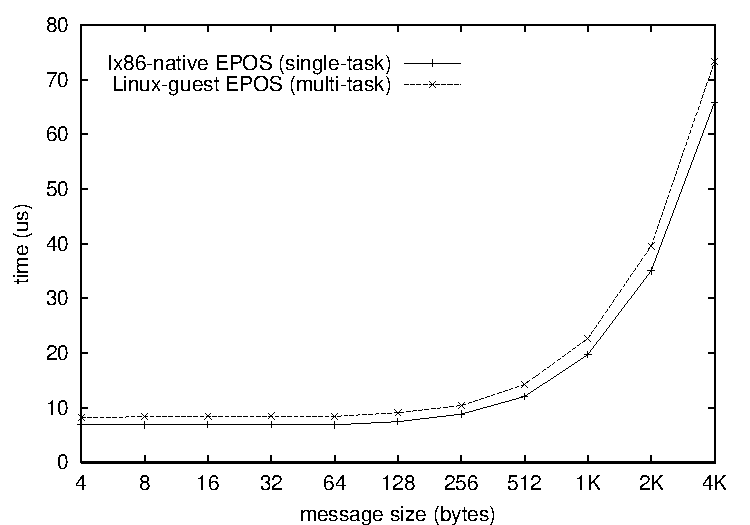
\includegraphics{fig/latency}}
    \resizebox*{\columnwidth}{!}{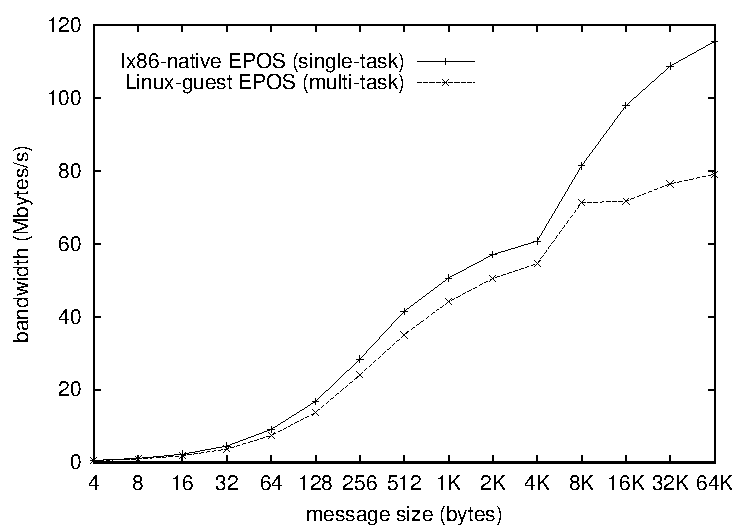
\includegraphics{fig/bandwidth}}
    \par
    \caption{\small{\texttt{Datagram}/\texttt{Port} one-way latency (left) and bandwidth (right).}}
    \label{fig:performance}
  \end{center}
\end{figure}

Even if the emulated version suffers from some additional overhead, the
native version showed significant performance improvements. This
advantage arises from the contiguous memory allocation method adopted,
which allows the DMA engines on the \textsc{Myrinet} card to be
programmed with logical addresses and eliminates the copy stage of the
pipeline (see figure
\ref{fig:pipeline}). This difference can be even more expressive if the
applications are multithread, since the copy stages of the pipeline
commence to concur with application threads for processor time and
specially for memory bandwidth. This can render our pipeline
architecture ineffective. Nevertheless, most parallel applications
execute on a single-task-per-node basis and will benefit from the
single-task versions of \textsc{Epos}. Other communication systems, such
as the Berkeley Active Messages~\cite{Lumetta:1997}, Illinois Fast
Messages~\cite{Pakin:1997}, Real World Computing Partnership
PM~\cite{Tezuka:1997}, and BIP~\cite{Prylli:1998}, run exclusively on
top of an ordinary operating system, such as \textsc{Unix} or
\textsc{Windows NT}, and have no alternative to escape this situation.

Furthermore, \textsc{Epos} quality evaluation is not restricted to
performance. Because only the components effectively required by the
applications are included, the resulting system is usually extremely
compact. The system in the example above, which in addition to
communication also includes process and memory management, has a size of
11 KBytes. This means less resource consumption and also less space for
bugs. Furthermore, \textsc{Epos} inflated interfaces try to preserve
fidelity to the problem domain, so that application programmers should
fell themselves comfortable to use them.


\section{Conclusion}

In this paper we applied \emph{Application-Oriented System Design} to
the design of a high-performance communication system for clusters. The
method prevented the monolithic conception of a generic solution in
favor of one that scales with application demands. The organization of
the corresponding problem domain in reusable components that can be
adapted to a given execution scenario and latter arranged in a framework
enable the system to be tailored to fulfill the requirements of specific
applications.

We also described the use of Application-Oriented System Design in the
\textsc{Epos} project, more specifically in its communication system,
which has been implemented for the \textsc{Myrinet} high-speed
network. This communication system consists of a collection of
\emph{application-ready, scenario-independent abstractions} (components)
that can be adapted to specific execution scenarios by means of
\emph{scenario-adapters} and can be arranged in a \emph{statically
metaprogrammed framework} to produce application-oriented communication
systems. The system is presented to application programmers through
\emph{inflated interfaces} that gather all variations of an abstraction
(family members) under a single, comprehensive and natural interface. By
programming based on these interfaces, programmers enable \textsc{Epos}
tools to automatically generate an adequate system for their
applications.

The results obtained so far are highly positive and help to corroborate
the guidelines of \emph{Application-Oriented System Design}, as well as
\textsc{Epos} design decisions. The evaluation of \textsc{Epos}
communication system revealed performance figures that, as far as we are
concerned, have no precedents in the \textsc{Myrinet} interconnected PC
cluster history. Nevertheless, \textsc{Epos} is a long term, open
project that aims at delivering application-oriented runtime systems to
a large universe of applications.


\bibliographystyle{plain}
\bibliography{se,os,network,cluster,guto}

\end{document}

%%% Local Variables: 
%%% mode: latex
%%% TeX-master: t
%%% End: 
